% ============================================================
% Echo Trail Ablation Study — Beamer Presentation
% J.C. Vaught — University of South Carolina
% ============================================================
\documentclass[aspectratio=169, 10pt]{beamer}

% ---- Packages ----
\usepackage[utf8]{inputenc}
\usepackage[T1]{fontenc}
\usepackage{lmodern}
\usepackage{graphicx}
\usepackage{booktabs}
\usepackage{amsmath, amssymb}
\usepackage{tikz}
\usepackage{pgfplots}
\pgfplotsset{compat=1.18}
\usetikzlibrary{arrows.meta, positioning, calc}
\usepackage{xcolor}
\usepackage{multicol}
\usepackage{array}

% ---- Graphics paths ----
\graphicspath{
  {../paper/figures/}
  {../paper/data/}
  {../paper/data/A1/}
  {../paper/data/A2/}
  {../path_previews/A1-4_preview/}
  {../path_previews/A5_preview/}
  {../path_previews/A6_preview/}
}

% ---- Brand Colors ----
\definecolor{Garnet}{RGB}{115, 0, 10}
\definecolor{Rose}{RGB}{204, 46, 64}
\definecolor{Atlantic}{RGB}{70, 106, 159}
\definecolor{Congaree}{RGB}{31, 65, 77}
\definecolor{Horseshoe}{RGB}{101, 120, 11}
\definecolor{Grass}{RGB}{206, 211, 24}
\definecolor{Honeycomb}{RGB}{164, 145, 55}
\definecolor{Black90}{RGB}{54, 54, 54}
\definecolor{Black70}{RGB}{92, 92, 92}
\definecolor{Black50}{RGB}{162, 162, 162}
\definecolor{Black30}{RGB}{199, 199, 199}
\definecolor{Black10}{RGB}{235, 235, 235}
\definecolor{WarmGrey}{RGB}{103, 97, 86}
\definecolor{Sandstorm}{RGB}{255, 242, 227}

% ---- Beamer Theme Setup ----
\usetheme{default}
\usecolortheme{default}
\setbeamertemplate{navigation symbols}{}
\setbeamertemplate{frametitle continuation}{}

% No rounded corners anywhere
\setbeamertemplate{blocks}[default]
\setbeamertemplate{items}[square]

% Colors
\setbeamercolor{structure}{fg=Garnet}
\setbeamercolor{frametitle}{fg=white, bg=Garnet}
\setbeamercolor{title}{fg=white, bg=Garnet}
\setbeamercolor{subtitle}{fg=Black70}
\setbeamercolor{author}{fg=Black90}
\setbeamercolor{date}{fg=Black70}
\setbeamercolor{institute}{fg=Black70}
\setbeamercolor{item}{fg=Garnet}
\setbeamercolor{subitem}{fg=Atlantic}
\setbeamercolor{normal text}{fg=Black90}
\setbeamercolor{block title}{fg=white, bg=Garnet}
\setbeamercolor{block body}{fg=Black90, bg=Black10}
\setbeamercolor{footline}{fg=Black50}

% Frame title formatting
\setbeamertemplate{frametitle}{%
  \nointerlineskip
  \begin{beamercolorbox}[wd=\paperwidth, ht=2.2em, dp=0.8em, leftskip=0.5cm]{frametitle}%
    \usebeamerfont{frametitle}\insertframetitle%
  \end{beamercolorbox}%
}

% Footer with slide numbers
\setbeamertemplate{footline}{%
  \hfill%
  \usebeamercolor[fg]{footline}%
  \footnotesize\insertframenumber\,/\,\inserttotalframenumber%
  \hspace{0.5cm}\vspace{0.3cm}%
}

% Font settings
\setbeamerfont{frametitle}{size=\large, series=\bfseries}
\setbeamerfont{title}{size=\Large, series=\bfseries}
\setbeamerfont{subtitle}{size=\normalsize}
\setbeamerfont{author}{size=\normalsize}
\setbeamerfont{institute}{size=\small}
\setbeamerfont{date}{size=\small}

% Custom commands
\newcommand{\maptf}{\text{mAP}_{50}}
\newcommand{\emphnum}[1]{\textcolor{Garnet}{\textbf{#1}}}
\newcommand{\keypoint}[1]{%
  \vfill
  \begin{beamercolorbox}[wd=\textwidth, dp=0.4em, leftskip=0.3cm]{block title}%
    \small #1%
  \end{beamercolorbox}%
}

% ============================================================
\begin{document}

% ============================================================
% SLIDE 1: TITLE
% ============================================================
{
\setbeamertemplate{footline}{}
\begin{frame}[plain]
\vspace{1.5cm}
\begin{beamercolorbox}[wd=\paperwidth, ht=3em, dp=1em, leftskip=1cm]{title}
  \usebeamerfont{title}Effect of Echo Trail Parameters on YOLO-Based\\
  Target Detection in Simulated Marine Radar Imagery
\end{beamercolorbox}
\vspace{0.8cm}
\begin{columns}[T]
\begin{column}{0.6\textwidth}
  \hspace{1cm}
  \begin{minipage}{0.9\textwidth}
    {\usebeamerfont{author}\usebeamercolor[fg]{author}J.C.\ Vaught}\\[0.3em]
    {\usebeamerfont{institute}\usebeamercolor[fg]{institute}University of South Carolina\\
    Advisors: Douglas Cahl, Yi Wang}\\[0.5em]
    {\usebeamerfont{date}\usebeamercolor[fg]{date}2026}
  \end{minipage}
\end{column}
\begin{column}{0.4\textwidth}
\end{column}
\end{columns}
\end{frame}
}

% ============================================================
% SECTION 1: INTRODUCTION
% ============================================================
\section{Introduction}

% ============================================================
% SLIDE 2: MOTIVATION
% ============================================================
\begin{frame}{Why Study Echo Trails?}

Echo trails render radar returns from previous antenna scans with progressively
reduced intensity. They appear on \textit{every} marine radar display.

\vspace{0.3cm}

\begin{itemize}
  \item IMO mandated trails on all shipborne radar in 2004 (MSC.192)
  \item No empirical study has examined how trail configuration affects ML detectors
  \item Same scene, different trail config $\rightarrow$ dramatically different detection outcomes
\end{itemize}

\vspace{0.3cm}

\begin{center}
  
\includegraphics[width=0.85\textwidth]{fig0_splash.pdf}
\end{center}

\keypoint{Trail rendering is not perceptually neutral for deep learning detectors.}
\end{frame}

% ============================================================
% SLIDE 3: RESEARCH QUESTIONS
% ============================================================
\begin{frame}{Research Questions and Contributions}

Eight sequential ablation experiments, each isolating one trail parameter.

\vspace{0.3cm}

\begin{columns}[T]
\begin{column}{0.48\textwidth}
  \textcolor{Garnet}{\textbf{Core Parameters}}
  \begin{enumerate}
    \item[\textbf{A1}] Trail length $N$ $\times$ target speed?
    \item[\textbf{A2}] Which decay function $f(k)$?
    \item[\textbf{A3}] Binary or proportional encoding?
    \item[\textbf{A4}] Which color mapping?
  \end{enumerate}
\end{column}
\begin{column}{0.48\textwidth}
  \textcolor{Atlantic}{\textbf{Environmental Factors}}
  \begin{enumerate}
    \item[\textbf{A5}] Range dependence of optimal $N$?
    \item[\textbf{A6}] Interaction with interference?
    \item[\textbf{A7}] Merging threshold for nearby targets?
    \item[\textbf{A8}] Crossing trajectory degradation?
  \end{enumerate}
\end{column}
\end{columns}

\vspace{0.5cm}

\textbf{Contribution:} First systematic investigation of echo trail parameters
on ML-based radar detection --- fills a 20+ year gap between regulatory mandate
and evidence-based optimization.

\end{frame}

% ============================================================
% SECTION 2: RADAR COMPOSITOR
% ============================================================
\section{Radar Compositor}

% ============================================================
% SLIDE 4: HARDWARE
% ============================================================
\begin{frame}{Target Hardware: Furuno DRS4D-NXT}

\begin{columns}[T]
\begin{column}{0.55\textwidth}
  X-band marine radar with the following specifications.

  \vspace{0.4cm}

  \begin{tabular}{@{}l r@{}}
    \toprule
    \textbf{Parameter} & \textbf{Value} \\
    \midrule
    Antenna RPM & 24 \\
    Pulses per revolution & 720 \\
    Azimuth resolution & 0.5\textdegree \\
    Range bins per pulse & 868 \\
    Maximum range & 3.0 nm \\
    Range resolution & $\sim$6.40 m/bin \\
    Native intensity & 4-bit (0--15) \\
    Processing intensity & 8-bit (0--255) \\
    PPI image size & 1735 $\times$ 1735 px \\
    \bottomrule
  \end{tabular}
\end{column}
\begin{column}{0.42\textwidth}
  \begin{center}
    \fbox{
\includegraphics[height=4.5cm,clip,trim=100 100 100 100]{../paper/data/A1/ppi/noclutter/N_0/frame_0030.png}}
  \end{center}
  {\small\centering Real PPI output (1735$\times$1735 px).}
\end{column}
\end{columns}

\keypoint{Our simulator matches this exact hardware specification.}
\end{frame}

% ============================================================
% SLIDE 5: CHARLESTON DATA
% ============================================================
\begin{frame}{Real-World Data Foundation: Charleston Harbor}

\begin{columns}[T]
\begin{column}{0.55\textwidth}
  Source: Furuno DRS4D-NXT recordings from Grice Marine Lab, Charleston SC.

  \vspace{0.4cm}

  \begin{tabular}{@{}l r@{}}
    \toprule
    \textbf{Dataset Component} & \textbf{Count} \\
    \midrule
    Background land frames & 280 \\
    Filtered target objects & 5,107 \\
    Interference objects & 4,642 \\
    Water/land annotation & 1 map \\
    \bottomrule
  \end{tabular}

  \vspace{0.4cm}

  Objects extracted via DBSCAN clustering (eps$=$3.0, min\_pts$=$3)
  on water-region radar returns. Each object stores a 2D echo
  pattern [pulse $\times$ range] with intensity, angular extent, and area.
\end{column}
\begin{column}{0.42\textwidth}
  \begin{center}
    
\includegraphics[height=4.5cm,clip,trim=50 30 50 30]{a1_scene_01.png}
  \end{center}
  {\small\centering Water mask with color-coded trajectories.}
\end{column}
\end{columns}

\keypoint{Real radar echoes ensure physically plausible target signatures.}
\end{frame}

% ============================================================
% SLIDE 6: PIPELINE OVERVIEW
% ============================================================
\begin{frame}{Six-Stage Synthetic Radar Pipeline}

\begin{center}
  
\includegraphics[width=0.9\textwidth]{fig_pipeline.pdf}
\end{center}

\vspace{0.3cm}

\begin{columns}[T]
\begin{column}{0.31\textwidth}
  \textcolor{Garnet}{\textbf{Generation}}
  \begin{enumerate}
    \item Data loading and validation
    \item Scene planning (trajectories)
  \end{enumerate}
\end{column}
\begin{column}{0.31\textwidth}
  \textcolor{Atlantic}{\textbf{Rendering}}
  \begin{enumerate}
    \setcounter{enumi}{2}
    \item CSV writing (polar + labels)
    \item Image rendering (Cartesian)
  \end{enumerate}
\end{column}
\begin{column}{0.31\textwidth}
  \textcolor{Congaree}{\textbf{Post-Processing}}
  \begin{enumerate}
    \setcounter{enumi}{4}
    \item Trail compositing
    \item Video export (optional)
  \end{enumerate}
\end{column}
\end{columns}

\keypoint{Trail rendering is a post-processing layer; all upstream parameters held constant across ablations.}
\end{frame}

% ============================================================
% SLIDE 7: OBJECT PLACEMENT
% ============================================================
\begin{frame}{Target Modeling: RCS-Based Object Placement}

\begin{columns}[T]
\begin{column}{0.55\textwidth}
  Objects from the Charleston library are placed onto background land frames
  via MAX-blending.

  \vspace{0.15cm}

  \textbf{Placement rule (per pixel):}
  \begin{equation*}
    \text{frame}[p][b] = \max\!\big(\text{current},\; \text{object echo}\big)
  \end{equation*}

  \vspace{0.05cm}

  \textbf{Intensity engine} controls per-frame scaling.
  \begin{itemize}\setlength{\itemsep}{0pt}
    \item Profiles: constant, ramp, sine, custom
    \item Variability: random jitter $\pm$10\% per frame
    \item Flicker: state machine for intermittent returns
  \end{itemize}

  \vspace{0.1cm}

  Objects inherit implicit RCS from real extraction --- no analytical radar
  equation required.
\end{column}
\begin{column}{0.42\textwidth}
  \begin{center}
    \fbox{
\includegraphics[height=2.5cm,clip,trim=100 100 100 100]{../paper/data/A1/ppi/noclutter/N_0/frame_0010.png}}~%
    \fbox{
\includegraphics[height=2.5cm,clip,trim=100 100 100 100]{../paper/data/A1/ppi/noclutter/N_10/frame_0010.png}}
  \end{center}
  {\small\centering Left: raw ($N{=}0$). Right: trails ($N{=}10$).}
\end{column}
\end{columns}

\keypoint{Real extracted echoes ensure physically plausible target signatures without analytical RCS models.}
\end{frame}

% ============================================================
% SLIDE 8: MOTION AND PATHS
% ============================================================
\begin{frame}{Target Motion: Speed Classes and Trajectories}

\begin{columns}[T]
\begin{column}{0.48\textwidth}
  \textbf{Three path types:}
  \begin{itemize}
    \item \textbf{Fixed} --- stationary (buoys, anchored vessels)
    \item \textbf{Linear} --- constant heading and speed
    \item \textbf{Bezier} --- smooth curved trajectories
  \end{itemize}

  \vspace{0.3cm}

  \textbf{Four speed classes:}

  \vspace{0.2cm}

  \begin{tabular}{@{}l r l@{}}
    \toprule
    \textbf{Class} & \textbf{Speed} & \textbf{Example} \\
    \midrule
    Stationary & 0 px/scan & Buoy \\
    Slow & 2 px/scan & Drift \\
    Medium & 5 px/scan & Cruising \\
    Fast & 15 px/scan & High-speed \\
    \bottomrule
  \end{tabular}
\end{column}
\begin{column}{0.48\textwidth}
  \begin{center}
    
\includegraphics[height=4.5cm,clip,trim=50 30 50 30]{a1_scene_01.png}
  \end{center}
  {\small\centering Stationary (white), slow (blue),\\medium (yellow), fast (red).}
\end{column}
\end{columns}

\keypoint{Speed parameterized in pixels/scan (not physical velocity) to capture range-dependent effects.}
\end{frame}

% ============================================================
% SLIDE 9: INTERFERENCE
% ============================================================
\begin{frame}{Radar Interference Simulation}

\begin{columns}[T]
\begin{column}{0.55\textwidth}
  Nearby X-band transmitters produce spoke-like artifacts on PPI displays.
  Our simulator models interference as synthetic radial streaks.

  \vspace{0.1cm}

  \textbf{Range-dependent geometry:}
  \begin{itemize}\setlength{\itemsep}{0pt}
    \item Azimuth width: $200 \cdot e^{-6r} + 5$ pulses
    \item Range length: $3 + 110r$ bins
    \item Raised-cosine intensity envelope
  \end{itemize}

  \vspace{0.05cm}

  \textbf{Configuration:}
  \begin{itemize}\setlength{\itemsep}{0pt}
    \item \texttt{num\_streaks}: 0--100+ per frame
    \item \texttt{intensity\_range}: [40,180] $\rightarrow$ [200,255]
    \item \texttt{per\_frame}: unique or shared seed
  \end{itemize}

  \vspace{0.05cm}

  4,642 real interference objects from Charleston recordings for validation.
\end{column}
\begin{column}{0.42\textwidth}
  \begin{center}
    \fbox{
\includegraphics[height=4.5cm,clip,trim=100 100 100 100]{../paper/data/A1/ppi/clutter/N_10/frame_0030.png}}
  \end{center}
  {\small\centering Interference streaks (red) overlay target returns (green).}
\end{column}
\end{columns}

\keypoint{Interference is the primary environmental confound for ML-based radar detection.}
\end{frame}

% ============================================================
% SLIDE 10: POLAR TO CARTESIAN
% ============================================================
\begin{frame}{Image Rendering: Polar to Cartesian Mapping}

\begin{columns}[T]
\begin{column}{0.55\textwidth}
  A precomputed lookup table (LUT) maps each Cartesian pixel to its
  polar source.

  \vspace{0.2cm}

  \textbf{For each pixel $(x, y)$:}
  \begin{align*}
    r &= \sqrt{dx^2 + dy^2}, \quad \theta = \text{atan2}(dx, dy) \\
    \text{pulse} &= \left\lfloor \frac{\theta}{2\pi} \cdot 720 \right\rfloor, \quad
    \text{bin} = \left\lfloor \frac{r}{r_{\max}} \cdot 868 \right\rfloor
  \end{align*}

  Only pixels with $r/r_{\max} \leq 1$ are valid (PPI circle).

  \vspace{0.2cm}

  \textbf{Label conversion:} Polar bounding boxes $\rightarrow$ axis-aligned
  Cartesian boxes via 4-corner transform.
\end{column}
\begin{column}{0.42\textwidth}
  \begin{center}
    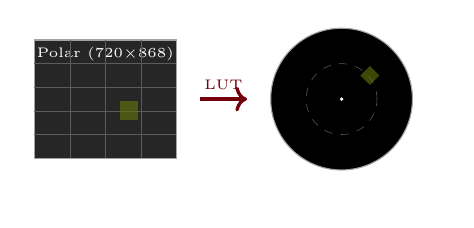
\begin{tikzpicture}[scale=0.6]
      % Polar frame (rectangle)
      \fill[black!85] (0,0) rectangle (3, 2.5);
      \draw[Black50] (0,0) rectangle (3, 2.5);
      \node[white, font=\tiny] at (1.5, 2.2) {Polar (720$\times$868)};
      % Grid lines
      \foreach \y in {0.5, 1.0, 1.5, 2.0} {
        \draw[Black70, very thin] (0, \y) -- (3, \y);
      }
      \foreach \x in {0.75, 1.5, 2.25} {
        \draw[Black70, very thin] (\x, 0) -- (\x, 2.5);
      }
      % Object in polar
      \fill[Horseshoe, opacity=0.6] (1.8, 0.8) rectangle (2.2, 1.2);
      % Arrow
      \draw[Garnet, very thick, ->] (3.5, 1.25) -- (4.5, 1.25);
      \node[Garnet, font=\tiny, above] at (4.0, 1.25) {LUT};
      % Cartesian PPI
      \begin{scope}[shift={(6.5, 1.25)}]
        \fill[black] (0,0) circle (1.5cm);
        \draw[Black50, thin] (0,0) circle (1.5cm);
        \draw[Black70, very thin, dashed] (0,0) circle (0.75cm);
        % Object in Cartesian (warped)
        \fill[Horseshoe, opacity=0.6] (0.6, 0.3) -- (0.8, 0.5) -- (0.6, 0.7) -- (0.4, 0.5) -- cycle;
        \fill[white] (0,0) circle (0.04cm);
        \node[white, font=\tiny] at (0, -1.8) {Cartesian (1735$\times$1735)};
      \end{scope}
    \end{tikzpicture}
  \end{center}
\end{column}
\end{columns}

\keypoint{Output matches what a human operator sees on a real radar display.}
\end{frame}

% ============================================================
% SLIDE 11: SCENE CONFIGS
% ============================================================
\begin{frame}{YAML-Driven Scene Generation}

\begin{columns}[T]
\begin{column}{0.48\textwidth}
  Each experiment defined by declarative YAML configuration files.

  \vspace{0.3cm}

  \begin{block}{Example Scene Config (condensed)}
    \ttfamily\scriptsize
    seed: 42\\
    count: 50\\
    objects:\\
    \ \ - name: stationary\\
    \ \ \ \ count: 15, size: [50, 300]\\
    \ \ \ \ path: \{type: fixed\}\\
    \ \ - name: fast\_edge\\
    \ \ \ \ count: 8, speed: 12.0\\
    \ \ \ \ path: \{type: linear\}\\
    clutter: \{num\_streaks: 100\}\\
    labels: \{export: true\}
  \end{block}
\end{column}
\begin{column}{0.48\textwidth}
  \textbf{Per ablation:}
  \begin{itemize}\setlength{\itemsep}{0pt}
    \item 10 scenes $\times$ 50 frames = 500 images
    \item 7 sub-classes $\rightarrow$ 2 classes (stationary, moving)
    \item YOLO format labels ($x_c$, $y_c$, $w$, $h$)
    \item Tested with and without interference
  \end{itemize}

  \vspace{0.15cm}

  \textbf{Ground truth counts:}

  \vspace{0.1cm}

  {\small\begin{tabular}{@{}l r@{}}
    \toprule
    \textbf{Class} & \textbf{Instances} \\
    \midrule
    Stationary & 750 \\
    Slow (2 px/scan) & 263 \\
    Medium (5 px/scan) & 216 \\
    Fast (15 px/scan) & 402 \\
    \bottomrule
  \end{tabular}}
\end{column}
\end{columns}

\keypoint{Full reproducibility --- every parameter specified declaratively.}
\end{frame}

% ============================================================
% SECTION 3: ECHO TRAIL RENDERING
% ============================================================
\section{Echo Trail Rendering}

% ============================================================
% SLIDE 12: COMPOSITING EQUATION
% ============================================================
\begin{frame}{Echo Trail Compositing: Per-Pixel MAX}

The displayed intensity at position $(r, \theta)$ at scan $t$ is the
maximum of decay-weighted historical returns.

\vspace{0.3cm}

\begin{center}
  \fcolorbox{Garnet}{Black10}{%
    \parbox{0.7\textwidth}{%
      \centering\vspace{0.2cm}
      $\displaystyle
        I_{\text{disp}}(r, \theta, t) = \max_{k=0}^{N} \Big[ f(k) \cdot I_{\text{raw}}(r, \theta, t{-}k) \Big]
      $
      \vspace{0.2cm}
    }%
  }
\end{center}

\vspace{0.3cm}

\begin{columns}[T]
\begin{column}{0.48\textwidth}
  \begin{itemize}
    \item $N$ = trail length (historical scans)
    \item $f(k)$ = decay function weighting scan $k$ ago
    \item $I_{\text{raw}}$ = raw intensity from scan $t{-}k$
  \end{itemize}
\end{column}
\begin{column}{0.48\textwidth}
  \begin{itemize}
    \item $\max$ operator: strong returns never attenuated
    \item Sliding window: each frame processes its own $N$-frame history
    \item No persistent state --- fully parallelizable
  \end{itemize}
\end{column}
\end{columns}

\keypoint{MAX compositing is consistent with real radar display behavior.}
\end{frame}

% ============================================================
% SLIDE 13: DECAY FUNCTIONS
% ============================================================
\begin{frame}{Four Decay Functions}

\begin{columns}[T]
\begin{column}{0.45\textwidth}
  \vspace{0.3cm}

  \textbf{Exponential:}
  $f(k) = e^{-k/\tau}$, \quad $\tau = \max(N/3,\, 1)$

  \vspace{0.3cm}

  \textbf{Concave:}
  $f(k) = \max\!\big(0,\; 1 - (k/N)^3\big)$

  \vspace{0.3cm}

  \textbf{Linear:}
  $f(k) = 1 - k/N$

  \vspace{0.3cm}

  \textbf{Step:}
  $f(k) = \begin{cases} 1 & k \leq N \\ 0 & k > N \end{cases}$

  \vspace{0.3cm}

  Each produces a different intensity profile for the trail streak behind
  a moving target.
\end{column}
\begin{column}{0.52\textwidth}
  \begin{center}
    
\includegraphics[width=\textwidth]{fig1_decay_functions.pdf}
  \end{center}
\end{column}
\end{columns}

\keypoint{Decay shape controls the visual contrast between target head and trail body.}
\end{frame}

% ============================================================
% SLIDE 14: INTENSITY ENCODING
% ============================================================
\begin{frame}{Intensity Encoding: Binary vs.\ Proportional}

\begin{columns}[T]
\begin{column}{0.48\textwidth}
  \textcolor{Garnet}{\textbf{Binary Encoding}}

  \vspace{0.2cm}

  Any non-zero return $\rightarrow$ full intensity:
  \[ w = \mathbb{1}[I > 0] \cdot f(k) \]

  \begin{itemize}
    \item High contrast, simple
    \item Loses amplitude (RCS) information
    \item A faint buoy and a large vessel produce identical trail pixels
  \end{itemize}
\end{column}
\begin{column}{0.48\textwidth}
  \textcolor{Atlantic}{\textbf{Proportional Encoding}}

  \vspace{0.2cm}

  Trail scales with original return strength:
  \[ w = (I / 255) \cdot f(k) \]

  \begin{itemize}
    \item Preserves radiometric information
    \item Fainter trails for weak targets
    \item Discriminative under interference
  \end{itemize}
\end{column}
\end{columns}

\vspace{0.1cm}

\begin{center}
  
\includegraphics[width=0.42\textwidth]{fig5_binary_proportional.pdf}
\end{center}

\keypoint{Binary maximizes contrast; proportional preserves amplitude --- each has a regime.}
\end{frame}

% ============================================================
% SLIDE 15: COLOR MAPPING
% ============================================================
\begin{frame}{Color Mapping: Four Strategies}

\begin{center}
  
\includegraphics[width=0.75\textwidth]{fig6_color_schemes.pdf}
\end{center}

\vspace{0.2cm}

\begin{columns}[T]
\begin{column}{0.24\textwidth}
  \centering
  \textcolor{Garnet}{\textbf{Monochrome}}\\
  {\small Green-on-black.\\Brightness = weight.}
\end{column}
\begin{column}{0.24\textwidth}
  \centering
  \textcolor{Atlantic}{\textbf{Two-tone}}\\
  {\small Current = green,\\history = red.}
\end{column}
\begin{column}{0.24\textwidth}
  \centering
  \textcolor{Horseshoe}{\textbf{Gradient}}\\
  {\small Age $\rightarrow$ hue ramp:\\green $\rightarrow$ red.}
\end{column}
\begin{column}{0.24\textwidth}
  \centering
  \textcolor{Congaree}{\textbf{Intensity}}\\
  {\small Return strength\\$\rightarrow$ hue (jet).}
\end{column}
\end{columns}

\keypoint{Color encodes temporal (age) or radiometric (strength) information --- functionally meaningful.}
\end{frame}

% ============================================================
% SLIDE 16: PARAMETER SPACE
% ============================================================
\begin{frame}{The Trail Parameter Space}

\begin{columns}[T]
\begin{column}{0.48\textwidth}
  Four independent parameters define a trail configuration.

  \vspace{0.3cm}

  \begin{tabular}{@{}l l r@{}}
    \toprule
    \textbf{Parameter} & \textbf{Options} & \textbf{Levels} \\
    \midrule
    Trail length $N$ & 0, 1, \ldots, 25 & 26 \\
    Decay $f(k)$ & exp, conc, lin, step & 4 \\
    Encoding & binary, proportional & 2 \\
    Color & mono, 2-tone, grad, int & 4 \\
    \midrule
    \multicolumn{2}{@{}l}{\textbf{Total configuration space}} & \textbf{832} \\
    \bottomrule
  \end{tabular}

  \vspace{0.4cm}

  Sequential ablation: optimize each in order, carry best forward.
  Reduces 832 configs to $\sim$46 training runs.
\end{column}
\begin{column}{0.48\textwidth}
  \begin{center}
    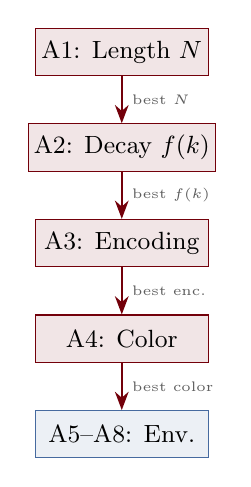
\begin{tikzpicture}[
      node distance=0.6cm,
      box/.style={draw=Garnet, fill=Garnet!10, minimum width=2.2cm,
                  minimum height=0.6cm, align=center, font=\small,
                  inner sep=2pt},
      arr/.style={->, >=Stealth, thick, Garnet}
    ]
      \node[box] (a1) {A1: Length $N$};
      \node[box, below=of a1] (a2) {A2: Decay $f(k)$};
      \node[box, below=of a2] (a3) {A3: Encoding};
      \node[box, below=of a3] (a4) {A4: Color};
      \node[box, below=of a4, fill=Atlantic!10, draw=Atlantic] (a58) {A5--A8: Env.};

      \draw[arr] (a1) -- (a2) node[midway, right, font=\tiny, Black70] {best $N$};
      \draw[arr] (a2) -- (a3) node[midway, right, font=\tiny, Black70] {best $f(k)$};
      \draw[arr] (a3) -- (a4) node[midway, right, font=\tiny, Black70] {best enc.};
      \draw[arr] (a4) -- (a58) node[midway, right, font=\tiny, Black70] {best color};
    \end{tikzpicture}
  \end{center}
\end{column}
\end{columns}

\keypoint{Each ablation isolates exactly one variable; best-of-prior carries forward.}
\end{frame}

% ============================================================
% SECTION 4: EXPERIMENTAL DESIGN
% ============================================================
\section{Experimental Design}

% ============================================================
% SLIDE 17: ABLATION STRUCTURE
% ============================================================
\begin{frame}{Sequential Ablation Design}

\begin{center}
\small
\begin{tabular}{@{}c l l l@{}}
  \toprule
  \textbf{Abl.} & \textbf{Variable} & \textbf{Levels Tested} & \textbf{Carries Forward} \\
  \midrule
  A1 & Trail length $\times$ speed & $N \in \{0,1,2,3,4,5,10,15,20,25\}$ & Best $N$ \\
  A2 & Decay function & exp, concave, linear, step & Best $f(k)$ \\
  A3 & Intensity encoding & binary, proportional & Best encoding \\
  A4 & Color mapping & mono, twotone, gradient, intensity & Best color \\
  \midrule
  A5 & Range dependence & near ($\sim$200m), mid ($\sim$1nm), far ($\sim$3nm) & --- \\
  A6 & Interference level & none, low, moderate, heavy & --- \\
  A7 & Target proximity & 10--100m separation & --- \\
  A8 & Crossing trajectories & 15\textdegree--90\textdegree\ crossing angle & --- \\
  \bottomrule
\end{tabular}
\end{center}

\vspace{0.3cm}

Each ablation tested under \textbf{two conditions}: clean and with interference.

\keypoint{A1--A4 optimize core parameters; A5--A8 test environmental robustness.}
\end{frame}

% ============================================================
% SLIDE 18: TRAINING PROTOCOL
% ============================================================
\begin{frame}{YOLOv8 Training Configuration}

\begin{columns}[T]
\begin{column}{0.48\textwidth}
  \textbf{Model and training:}
  \begin{itemize}
    \item YOLOv8-nano, COCO pretrained
    \item 50 epochs, $\text{lr}_0 = 1 \times 10^{-3}$
    \item Batch size 16, input 640$\times$640
    \item Standard augmentation (flip, mosaic, mixup)
    \item Seed 42, deterministic
  \end{itemize}

  \vspace{0.3cm}

  \textbf{Dataset per condition:}
  \begin{itemize}
    \item 10 scenes $\times$ 50 frames = 500 images
    \item Train: scenes 1--9 (450 images)
    \item Validation: scene 10 (50 images)
  \end{itemize}
\end{column}
\begin{column}{0.48\textwidth}
  \textbf{Detection classes:}

  \vspace{0.2cm}

  \begin{tabular}{@{}l l@{}}
    \toprule
    \textbf{Class} & \textbf{Sub-classes} \\
    \midrule
    0: stationary & stationary \\
    1: moving & slow, medium, fast \\
    \bottomrule
  \end{tabular}

  \vspace{0.4cm}

  Independent training per condition --- no information leakage between
  ablation levels.

  \vspace{0.3cm}

  Intentionally small dataset (450 images) reflects data-limited
  specialized radar applications.
\end{column}
\end{columns}

\keypoint{Independent training per condition ensures no information leakage between ablation levels.}
\end{frame}

% ============================================================
% SLIDE 19: METRICS
% ============================================================
\begin{frame}{Evaluation Metrics}

\begin{columns}[T]
\begin{column}{0.55\textwidth}
  \textbf{Primary metric:} $\maptf$ (mAP at IoU $\geq$ 0.50)

  \vspace{0.2cm}

  \textbf{Secondary:} $\text{mAP}_{50\text{-}95}$, precision, recall, F1

  \vspace{0.3cm}

  \textbf{Speed-tier stratification:} metrics computed separately for
  stationary, slow, medium, and fast targets to isolate kinematics effects.

  \vspace{0.3cm}

  \textbf{Why $\maptf$?}
  \begin{itemize}
    \item Conservative (lenient on box geometry)
    \item Trail streaks enlarge predicted boxes, reducing IoU
    \item Stricter thresholds would show even larger trail-induced degradation
  \end{itemize}
\end{column}
\begin{column}{0.42\textwidth}
  \begin{center}
    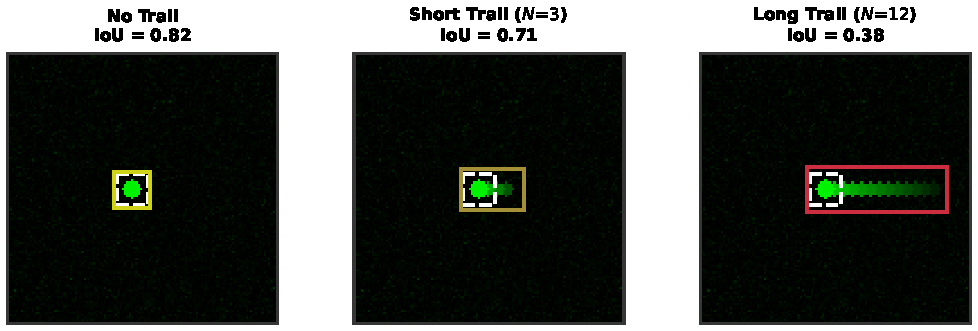
\includegraphics[width=0.95\textwidth]{fig_iou.pdf}
  \end{center}
  \vspace{0.1cm}
  {\small Trail streaks distort predicted bounding boxes, systematically
  degrading IoU with ground truth.}
\end{column}
\end{columns}

\keypoint{$\maptf$ chosen as primary metric; stricter thresholds would amplify trail-induced degradation.}
\end{frame}

% ============================================================
% SECTION 5: RESULTS
% ============================================================
\section{Results}

% ============================================================
% SLIDE 20: A1 NO-CLUTTER
% ============================================================
\begin{frame}{E1: Trail Length $\times$ Speed (No Interference)}

\begin{columns}[T]
\begin{column}{0.48\textwidth}
  Overall $\maptf$: monotonic rise from \emphnum{0.675} ($N{=}0$) to
  \emphnum{0.918} ($N{=}25$).

  \vspace{0.2cm}

  \textbf{By speed tier:}
  \begin{itemize}\setlength{\itemsep}{0pt}
    \item \textbf{Stationary:} 0.339 $\rightarrow$ 0.793 ($N{=}20$)
    \item \textbf{Slow:} 0.449 $\rightarrow$ 0.778 ($N{=}25$), non-monotonic
    \item \textbf{Medium:} 0.431 $\rightarrow$ 0.848 ($N{=}25$), erratic
    \item \textbf{Fast:} \emphnum{+34.7pp} jump at $N{=}3$, saturated by $N{=}10$
  \end{itemize}

  \vspace{0.1cm}

  Steep gain: +17pp ($N{=}0$ to $N{=}4$); diminishing after.
\end{column}
\begin{column}{0.50\textwidth}
  \begin{center}
    
\includegraphics[width=\textwidth]{fig3_trail_length_speed.pdf}
  \end{center}
\end{column}
\end{columns}

\keypoint{Fast targets benefit explosively from even short trails; stationary targets need $N{=}$10--15.}
\end{frame}

% ============================================================
% SLIDE 21: A1 CLUTTER
% ============================================================
\begin{frame}{E1: Trail Length $\times$ Speed (With Interference)}

\begin{columns}[T]
\begin{column}{0.48\textwidth}
  Overall $\maptf$: peaks at \emphnum{0.720} ($N{=}15$), then
  \textbf{regresses to 0.669 at $N{=}25$} --- below baseline.

  \vspace{0.2cm}

  \textbf{By speed tier (interference):}
  \begin{itemize}
    \item \textbf{Stationary:} peaks at $N{=}3$ (0.580)
    \item \textbf{Slow:} \textcolor{Rose}{\textbf{catastrophic failure}} --- peaks at $N{=}1$ (0.383), collapses to 0.207 at $N{=}25$
    \item \textbf{Medium:} peaks at $N{=}15$ (0.446)
    \item \textbf{Fast:} stable 0.468--0.568
  \end{itemize}

  \vspace{0.2cm}

  Slow-target recall drops from 0.681 ($N{=}0$) to 0.491 ($N{=}25$)
  --- loss of \emphnum{19pp}.
\end{column}
\begin{column}{0.50\textwidth}
  \begin{center}
    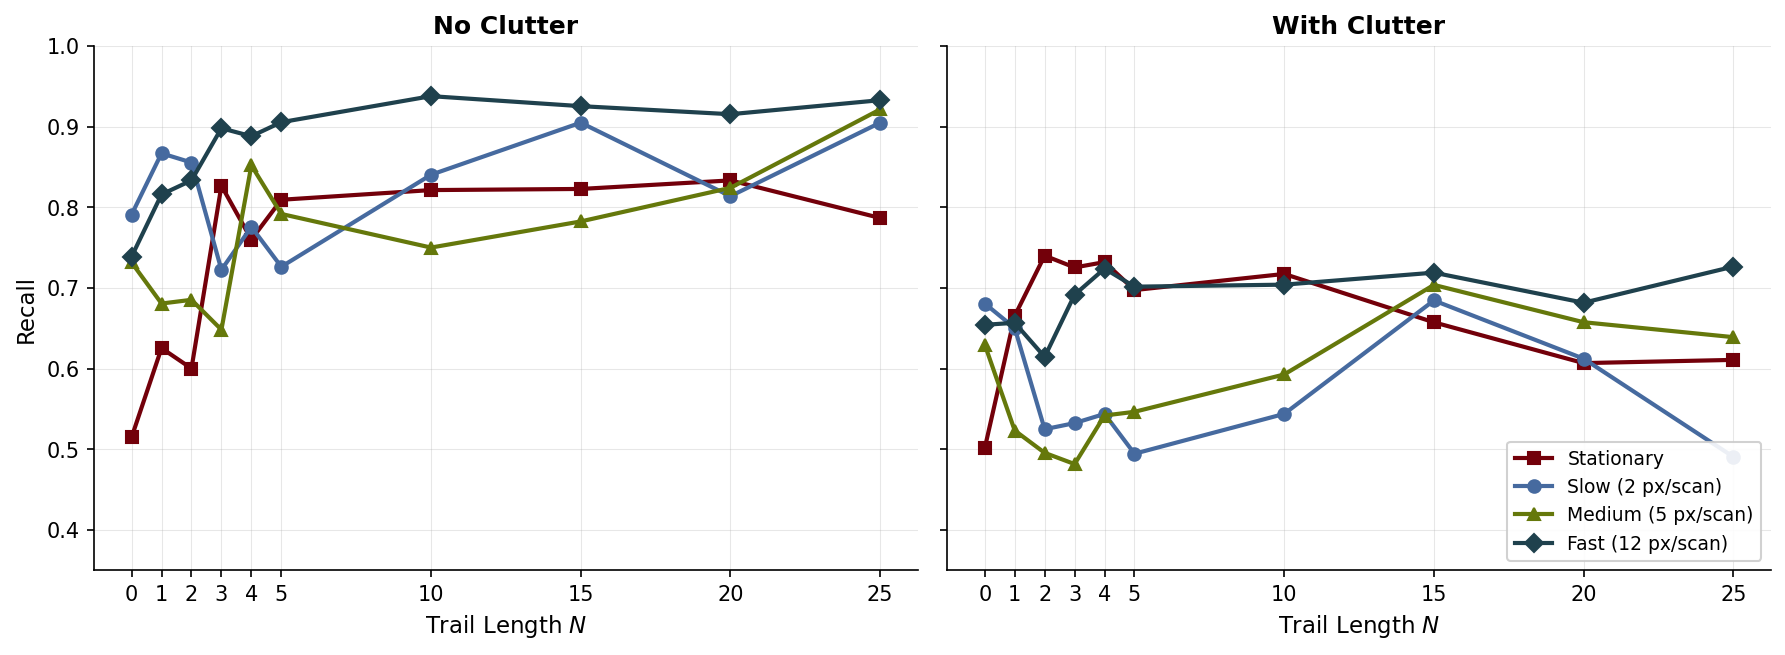
\includegraphics[width=\textwidth]{speed_tier_recall_both.png}
  \end{center}
\end{column}
\end{columns}

\keypoint{Longer trails that help clean scenes \textit{actively harm} slow targets under interference.}
\end{frame}

% ============================================================
% SLIDE 22: CLUTTER GAP
% ============================================================
\begin{frame}{E1: The Interference Gap Widens with Trail Length}

\begin{columns}[T]
\begin{column}{0.50\textwidth}
  \textbf{Interference gap} = (clean $\maptf$) $-$ (interference $\maptf$)

  \vspace{0.3cm}

  \begin{tabular}{@{}c c c c@{}}
    \toprule
    $N$ & Clean & Interf. & \textbf{Gap} \\
    \midrule
    0 & 0.675 & 0.671 & 0.004 \\
    5 & 0.844 & 0.673 & 0.171 \\
    10 & 0.891 & 0.691 & 0.200 \\
    15 & 0.899 & 0.720 & 0.179 \\
    25 & 0.918 & 0.669 & \textcolor{Rose}{\textbf{0.249}} \\
    \bottomrule
  \end{tabular}

  \vspace{0.3cm}

  Trail representation that benefits clean scenes is \textit{most distorted}
  by interference.
\end{column}
\begin{column}{0.48\textwidth}
  \textbf{Optimal $N$ depends on environment:}

  \vspace{0.3cm}

  \begin{block}{Clean conditions}
    $N{=}10$--15 captures $\sim$97\% of achievable gain.
  \end{block}

  \vspace{0.2cm}

  \begin{block}{With interference}
    Never exceed $N{=}15$. For slow targets: $N{=}1$ or none.
  \end{block}

  \vspace{0.3cm}

  No single trail length is universally optimal.
\end{column}
\end{columns}

\keypoint{Trail configuration must be adapted to environmental conditions.}
\end{frame}

% ============================================================
% SLIDE 23: A2 DECAY
% ============================================================
\begin{frame}{E2: Decay Function Comparison}

\begin{columns}[T]
\begin{column}{0.45\textwidth}
  \textbf{Clean ranking:}\\
  Exp (0.898) $>$ Conc (0.892) $>$ Lin (0.891) $>$ Step (0.885)

  \vspace{0.3cm}

  \textbf{Interference ranking:}\\
  \textcolor{Rose}{\textbf{Step (0.700)}} $>$ Exp (0.691) $\approx$ Lin (0.691) $>$ Conc (0.669)

  \vspace{0.3cm}

  \textcolor{Garnet}{\textbf{Complete rank inversion.}}

  \vspace{0.3cm}

  \begin{tabular}{@{}l c@{}}
    \toprule
    \textbf{Function} & \textbf{Relative Drop} \\
    \midrule
    Step & 20.9\% (most robust) \\
    Exponential & 23.0\% \\
    Linear & 22.5\% \\
    Concave & 24.9\% (worst) \\
    \bottomrule
  \end{tabular}
\end{column}
\begin{column}{0.52\textwidth}
  \begin{center}
    
\includegraphics[width=\textwidth]{fig4_decay_shape.pdf}
  \end{center}
\end{column}
\end{columns}

\keypoint{Exponential for clean conditions; step for interference; avoid concave operationally.}
\end{frame}

% ============================================================
% SLIDE 24: A3 ENCODING
% ============================================================
\begin{frame}{E3: Binary vs.\ Proportional Intensity}

\begin{columns}[T]
\begin{column}{0.48\textwidth}
  \begin{center}
    
\includegraphics[width=0.95\textwidth]{fig5_binary_proportional.pdf}
  \end{center}
\end{column}
\begin{column}{0.48\textwidth}
  \textbf{Clean:} Binary leads \emphnum{+3.45pp}\\
  (0.872 vs.\ 0.837)

  \vspace{0.3cm}

  \textbf{Interference:} Proportional leads +0.34pp\\
  (0.657 vs.\ 0.653)

  \vspace{0.3cm}

  \textbf{Interference fragility:}
  \begin{itemize}
    \item Binary: \textcolor{Rose}{21.8pp} penalty
    \item Proportional: 18.1pp penalty
  \end{itemize}

  \vspace{0.3cm}

  \textbf{Moving targets show sharpest reversal:}\\
  Binary +4.85pp clean $\rightarrow$ proportional +2.50pp with interference.

  \vspace{0.2cm}

  {\small Amplitude gradients become discriminative when interference
  contaminates at uniform intensity.}
\end{column}
\end{columns}

\keypoint{Binary wins clean (+3.45pp); proportional is more interference-robust (18.1pp vs 21.8pp penalty).}
\end{frame}

% ============================================================
% SLIDE 25: A4 COLOR
% ============================================================
\begin{frame}{E4: Color Mapping Strategies}

\begin{columns}[T]
\begin{column}{0.48\textwidth}
  \textbf{Clean ranking:}\\
  Gradient (0.871) $>$ Twotone (0.837)\\
  $>$ Intensity (0.810) $>$ Mono (0.736)

  \vspace{0.3cm}

  \textbf{Interference ranking:}\\
  Intensity (0.670) $>$ Gradient (0.667)\\
  $>$ Twotone (0.657) $>$ Mono (0.576)

  \vspace{0.3cm}

  \textcolor{Garnet}{\textbf{Any color encoding outperforms mono by 9--13+ $\maptf$ points.}}

  \vspace{0.3cm}

  \begin{tabular}{@{}l c@{}}
    \toprule
    \textbf{Scheme} & \textbf{Interf.\ Robustness} \\
    \midrule
    Intensity & 17.2\% drop (best) \\
    Twotone & 21.6\% drop \\
    Mono & 21.8\% drop \\
    Gradient & 23.4\% drop (worst) \\
    \bottomrule
  \end{tabular}
\end{column}
\begin{column}{0.50\textwidth}
  \begin{center}
    
\includegraphics[width=\textwidth]{fig6_color_schemes.pdf}
  \end{center}
\end{column}
\end{columns}

\keypoint{Color mapping is functionally meaningful --- not cosmetic decoration.}
\end{frame}

% ============================================================
% SLIDE 26: A5 RANGE
% ============================================================
\begin{frame}{E5: Range-Dependent Trail Optimization}

\begin{columns}[T]
\begin{column}{0.48\textwidth}
  Same physical speed produces different pixel displacement at different ranges.

  \vspace{0.3cm}

  \begin{tabular}{@{}l c c@{}}
    \toprule
    \textbf{Range} & \textbf{Bin} & \textbf{Optimal $N$} \\
    \midrule
    Near ($\sim$200m) & $\sim$80 & $\approx$ 3 \\
    Mid ($\sim$1 nm) & $\sim$350 & $\approx$ 10 \\
    Far ($\sim$3 nm) & $\sim$750 & $\approx$ 24 \\
    \bottomrule
  \end{tabular}

  \vspace{0.3cm}

  A single fixed trail length cannot optimize detection across all ranges
  simultaneously.

  \vspace{0.3cm}

  \textbf{Solution:} Range-adaptive trail rendering --- vary $N$ as a
  function of range within a single PPI frame.
\end{column}
\begin{column}{0.50\textwidth}
  \begin{center}
    
\includegraphics[width=\textwidth]{fig7_range_dependence.pdf}
  \end{center}
\end{column}
\end{columns}

\keypoint{Range-adaptive rendering: short trails near, long trails far.}
\end{frame}

% ============================================================
% SLIDE 27: A6 CLUTTER INTERACTION
% ============================================================
\begin{frame}{E6: Trail-Interference Interaction}

\begin{columns}[T]
\begin{column}{0.48\textwidth}
  \begin{center}
    
\includegraphics[width=0.95\textwidth]{fig8_clutter.pdf}
  \end{center}
\end{column}
\begin{column}{0.48\textwidth}
  Trails provide the greatest benefit under heavy interference.

  \vspace{0.2cm}

  \textbf{Mechanism:} Temporal signal integration accumulates
  target returns above the fluctuating interference floor.

  \vspace{0.2cm}

  \begin{itemize}\setlength{\itemsep}{0pt}
    \item \textbf{Low interf.:} modest benefit (strong SNR)
    \item \textbf{Heavy interf.:} baseline degrades; trails help via accumulation
  \end{itemize}

  \vspace{0.2cm}

  Speed-dependent: fast targets gain, slow targets may degrade. Interference inverts stationary/moving ranking for all A1--A4 configs.
\end{column}
\end{columns}

\keypoint{Trails help most under heavy interference, but the benefit is speed-dependent.}
\end{frame}

% ============================================================
% SLIDE 28: A7 MERGING
% ============================================================
\begin{frame}{E7: Target Proximity and Merging Threshold}

\begin{columns}[T]
\begin{column}{0.48\textwidth}
  \begin{center}
    
\includegraphics[width=0.95\textwidth]{fig9_merging.pdf}
  \end{center}
\end{column}
\begin{column}{0.48\textwidth}
  Two stationary targets at varying separations (10--100m).

  \vspace{0.3cm}

  \textbf{Without trails ($N{=}0$):}\\
  Targets resolve down to $\sim$\emphnum{20m} separation.

  \vspace{0.3cm}

  \textbf{With trails ($N{=}12$):}\\
  Merging threshold shifts to $\sim$\emphnum{28m}.

  \vspace{0.3cm}

  \textbf{An 8m increase} in minimum resolvable separation due to trail
  spatial footprint expansion.

  \vspace{0.3cm}

  Operationally significant in dense target environments: harbors,
  buoy fields, congested waterways.
\end{column}
\end{columns}

\keypoint{Trails improve individual detection but degrade discrimination of nearby targets.}
\end{frame}

% ============================================================
% SLIDE 29: A8 CROSSING
% ============================================================
\begin{frame}{E8: Crossing Trajectory Overlap}

\begin{columns}[T]
\begin{column}{0.48\textwidth}
  Two moving targets on converging paths at various crossing angles.

  \vspace{0.3cm}

  \textbf{Shallow angles ($<$30\textdegree):}\\
  Severe degradation --- trails overlap extensively, creating a single
  elongated artifact.

  \vspace{0.3cm}

  \textbf{90\textdegree\ crossing:}\\
  Minimal overlap --- trails point in perpendicular directions, resolvable.

  \vspace{0.3cm}

  \textbf{Decay function matters:}
  \begin{itemize}
    \item \textbf{Step:} uniform-intensity overlap zone (maximally confusing)
    \item \textbf{Exponential:} faint tail overlap (detector may still resolve)
  \end{itemize}
\end{column}
\begin{column}{0.50\textwidth}
  \begin{center}
    
\includegraphics[width=\textwidth]{fig10_crossing.pdf}
  \end{center}
\end{column}
\end{columns}

\keypoint{Shallow-angle crossings with long trails are the worst case for multi-target detection.}
\end{frame}

% ============================================================
% SLIDE 30: KEY FINDINGS (A1-A4)
% ============================================================
\begin{frame}{Key Findings (A1--A4)}

\begin{itemize}\setlength{\itemsep}{4pt}
  \item Trail rendering shifts $\maptf$ by \emphnum{3--25pp} --- not cosmetic,
        it is an input transformation for the detector.

  \item \textbf{No single configuration wins:} the optimal setting flips between
        clean and cluttered conditions for every parameter.

\end{itemize}

\vspace{0.15cm}

\begin{center}
\small
\begin{tabular}{@{}l c c@{}}
  \toprule
  \textbf{Experiment} & \textbf{Best (Clean)} & \textbf{Best (Interference)} \\
  \midrule
  A1: Trail Length      & $N{=}25$ (0.918) & $N{=}15$ (0.720) \\
  A2: Decay Function    & Exponential (0.898) & Step (0.700) \\
  A3: Intensity Encoding & Binary (0.872) & Proportional (0.657) \\
  A4: Color Mapping     & Gradient (0.871) & Intensity (0.670) \\
  \bottomrule
\end{tabular}
\end{center}

\vspace{0.15cm}

\begin{itemize}\setlength{\itemsep}{4pt}
  \item Any color encoding $\gg$ monochrome (\emphnum{+9--13pp}) --- largest single effect.
  \item Interference \textit{universally} inverts the stationary/moving ranking across all experiments.
\end{itemize}

\keypoint{Optimizing for clean scenes actively degrades performance under interference.}
\end{frame}

% ============================================================
% SLIDE 31: SURPRISING RESULTS
% ============================================================
\begin{frame}{Surprising Results}

\begin{enumerate}\setlength{\itemsep}{4pt}
  \item \textbf{Longer trails can \textit{hurt}:} at $N{=}25$ with interference,
        $\maptf$ (\emphnum{0.669}) drops \textit{below} the no-trail baseline (0.671).
        Slow targets collapse from 0.383 ($N{=}1$) to 0.207 ($N{=}25$).

  \item \textbf{Fast targets saturate by $N{=}3$:} +34.7pp jump
        ($0.488 \to 0.836$), barely improve after. Long trails are wasted on fast targets.

  \item \textbf{Binary/proportional encoding reverses under interference:}
        binary leads +3.45pp clean, but proportional is more robust
        (18.1pp penalty vs.\ 21.8pp). Uniform-intensity clutter becomes a
        discriminative cue only under proportional encoding.

  \item \textbf{Medium-speed targets always hardest} ($\sim$0.24--0.34 $\maptf$)
        across every experiment. Too fast for buildup, too slow to streak.

  \item \textbf{Zero false positives on moving targets} at every trail length.
        Precision = 1.0; all errors are missed detections.
\end{enumerate}

\keypoint{Trail rendering interacts with detection in non-obvious, speed-dependent ways.}
\end{frame}

% ============================================================
% SLIDE 32 (was 30 cont.): SUMMARY TABLE + HEATMAP
% ============================================================
\begin{frame}{Summary: All Ablations at a Glance}

\begin{center}
\small
\begin{tabular}{@{}c l c c l@{}}
  \toprule
  & \textbf{Variable} & \textbf{Best (Clean)} & \textbf{Best (Interf.)} & \textbf{Key Finding} \\
  \midrule
  A1 & Length $N$ & $N{=}25$ (0.918) & $N{=}15$ (0.720) & Fast saturate by $N{=}3$ \\
  A2 & Decay $f(k)$ & Exp (0.898) & Step (0.700) & Complete rank inversion \\
  A3 & Encoding & Binary (0.872) & Prop (0.657) & Amplitude cue under interf. \\
  A4 & Color & Gradient (0.871) & Intensity (0.670) & Any color $\gg$ mono \\
  \midrule
  A5 & Range & Near: $N{\approx}3$ & Far: $N{\approx}24$ & Range-adaptive needed \\
  A6 & Interference & \multicolumn{2}{c}{Trails help heavy interf.} & Slow targets persist \\
  A7 & Proximity & $\sim$20m & $\sim$28m & +8m merging shift \\
  A8 & Crossing & 90\textdegree\ OK & $<$30\textdegree\ fails & Shallow angles degrade \\
  \bottomrule
\end{tabular}
\end{center}

\vspace{0.15cm}

\begin{center}
  
\includegraphics[width=0.45\textwidth]{fig11_summary_heatmap.pdf}
\end{center}

\keypoint{No single configuration dominates --- optimal trails depend on speed, range, and interference.}
\end{frame}

% ============================================================
% SECTION 6: DISCUSSION AND CONCLUSION
% ============================================================
\section{Discussion and Conclusion}

% ============================================================
% SLIDE 32: RECOMMENDATIONS
% ============================================================
\begin{frame}{Operational Recommendations}

\begin{columns}[T]
\begin{column}{0.48\textwidth}
  \textcolor{Garnet}{\textbf{Trail Configuration}}
  \begin{enumerate}
    \item No single $N$ is optimal. Fast: $N{=}3$. Stationary: $N{=}10$--15. Slow in interference: $N{\leq}1$.
    \item Exp.\ decay for clean; step for interference. Avoid concave.
    \item Proportional encoding for high-interference environments.
    \item Always use color encoding (any scheme beats mono by 9--13pp).
  \end{enumerate}
\end{column}
\begin{column}{0.48\textwidth}
  \textcolor{Atlantic}{\textbf{System Design}}
  \begin{enumerate}
    \setcounter{enumi}{4}
    \item Range-adaptive trail rendering: short $N$ near, long $N$ far.
    \item Avoid long trails in dense environments (+8m merging shift).
    \item Slow targets in interference need upstream CFAR / coherent integration.
  \end{enumerate}
\end{column}
\end{columns}

\keypoint{Actionable guidelines for radar system designers integrating ML detection.}
\end{frame}

% ============================================================
% SLIDE 33: STRUCTURAL LIMITATIONS
% ============================================================
\begin{frame}{The Slow-Target Floor and Other Limits}

\begin{columns}[T]
\begin{column}{0.55\textwidth}
  \textbf{Slow targets in interference:}\\
  $\sim$\emphnum{0.31 $\maptf$} ceiling across ALL configurations.

  \vspace{0.2cm}

  This is a \textit{structural limitation} of trail augmentation, not a
  parameter tuning problem.

  \vspace{0.2cm}

  \textbf{Root cause:} slow targets produce small displacements that trails
  mix into accumulated interference returns.

  \vspace{0.2cm}

  \textbf{Additional limits:}
  \begin{itemize}
    \item Precision globally low (max 0.470)
    \item Medium-speed tier consistently hardest
    \item Trails increase bbox size for moving targets
  \end{itemize}
\end{column}
\begin{column}{0.42\textwidth}
  \begin{center}
    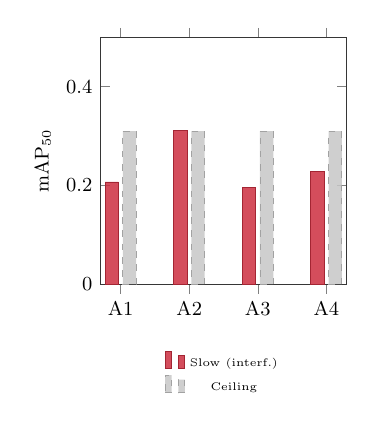
\begin{tikzpicture}[scale=0.8]
      \begin{axis}[
        width=5.5cm, height=5.5cm,
        ybar, bar width=6pt,
        ymin=0, ymax=0.5,
        ylabel={$\maptf$},
        ylabel style={font=\small},
        xlabel style={font=\small},
        symbolic x coords={A1, A2, A3, A4},
        xtick=data,
        tick label style={font=\small},
        axis line style={Black90},
        legend style={at={(0.5,-0.25)}, anchor=north, font=\tiny, draw=none},
        every axis plot/.append style={fill opacity=0.85}
      ]
        \addplot[fill=Rose, draw=Rose!80!black]
          coordinates {(A1, 0.207) (A2, 0.311) (A3, 0.196) (A4, 0.228)};
        \addplot[fill=Black30, draw=Black50, dashed]
          coordinates {(A1, 0.31) (A2, 0.31) (A3, 0.31) (A4, 0.31)};
        \legend{Slow (interf.), Ceiling}
      \end{axis}
    \end{tikzpicture}
  \end{center}
  {\small\centering Slow-target performance never exceeds $\sim$0.31 regardless
  of trail configuration.}
\end{column}
\end{columns}

\keypoint{Some detection challenges cannot be solved at the display layer.}
\end{frame}

% ============================================================
% SLIDE 34: FUTURE WORK
% ============================================================
\begin{frame}{Future Directions}

\begin{columns}[T]
\begin{column}{0.48\textwidth}
  \textcolor{Garnet}{\textbf{Validation and Extension}}
  \begin{enumerate}
    \item Validate on real Furuno DRS4D-NXT recordings from Charleston Harbor
    \item Extend to other architectures (Faster R-CNN, DETR, transformers)
    \item Real-time range-adaptive trail rendering implementation
  \end{enumerate}
\end{column}
\begin{column}{0.48\textwidth}
  \textcolor{Atlantic}{\textbf{Deeper Investigation}}
  \begin{enumerate}
    \setcounter{enumi}{3}
    \item Trail-tracking interaction (Kalman filters, Hungarian algorithm)
    \item Detector confidence calibration under different trail configs
    \item Upstream interference suppression (CFAR, MTI) before trail rendering
    \item Color similarity threshold --- minimum hue separation for discrimination
  \end{enumerate}
\end{column}
\end{columns}

This work establishes the empirical foundation. Operational deployment requires
hardware validation and integration with full radar signal processing chains.

\keypoint{Immediate next step: validate synthetic findings on real Furuno DRS4D-NXT recordings.}
\end{frame}

% ============================================================
% SLIDE 35: QUESTIONS
% ============================================================
{
\setbeamertemplate{footline}{}
\begin{frame}[plain]
\vfill
\begin{beamercolorbox}[wd=\paperwidth, ht=3em, dp=1em, leftskip=1cm]{title}
  \usebeamerfont{title}Questions?
\end{beamercolorbox}
\vfill
\begin{center}
  {\large J.C.\ Vaught}\\[0.3em]
  {\normalsize jvaught@sc.edu}\\[0.3em]
  {\small University of South Carolina}\\[0.5em]
  {\footnotesize Paper submitted to IDETC 2026}
\end{center}
\vfill
\end{frame}
}

\end{document}
